\documentclass[compress,aspectratio=169]{beamer}
\usepackage{ragged2e}
\usepackage{underscore}
%Setup File
% \usepackage[english]{babel}
\usepackage[brazilian]{babel}
\usepackage[letterpaper,top=2cm,bottom=2cm,left=3cm,right=3cm,marginparwidth=1.75cm]{geometry}

% Useful packages
\usepackage{amsmath}
\usepackage{graphicx}
% \usepackage[colorlinks=true,linkcolor=blue]{hyperref}
\usepackage{hyperref}
\usepackage{listings}
\usepackage[figure,table,lstlisting]{totalcount}
\usepackage{tcolorbox}
\usepackage{listings}
\usepackage{xcolor}

\usepackage[parfill]{parskip}

\hypersetup{
    colorlinks=true,
    linkcolor=black,
    filecolor=magenta,      
    urlcolor=cyan,
    pdftitle={Overleaf Example},
    pdfpagemode=FullScreen,
    }

\definecolor{verde}{rgb}{0.25,0.5,0.35}
\definecolor{jpurple}{rgb}{0.5,0,0.35}

\lstset{
  language=C++,
  basicstyle=\ttfamily\small,
  keywordstyle=\color{jpurple}\bfseries,
  stringstyle=\color{red},
  commentstyle=\color{verde},
  morecomment=[s][\color{blue}]{/**}{*/},
  extendedchars=true,
  showspaces=false,
  showstringspaces=false,
  numbers=left,
  numberstyle=\tiny,
  breaklines=true,
  backgroundcolor=\color{cyan!10},
  breakautoindent=true,
  captionpos=b,
  xleftmargin=0pt,
  tabsize=4
}

\renewcommand{\lstlistingname}{Código}
\renewcommand{\lstlistlistingname}{Lista de Códigos Fonte}

\newcommand\conditionalLoF{%
    \iftotalfigures
        \listoffigures
    \fi}
\newcommand\conditionalLoT{%
    \iftotaltables
        \listoftables
    \fi}
\newcommand\conditionalLoL{%
    \iftotallstlistings
        \lstlistoflistings
    \fi}

\newcommand{\DESCRICAO}[1]{
    % set flexible interword space
    \setlength{\spaceskip}{0.5em plus 1em minus 0.1em}%
    % add some space with not as much flexibility, but only
    % if some space precedes
    \ifdim\lastskip>0pt \hspace{0.5em plus 0.5em minus 0.1em}\fi
    \texttt{\textbf{\color{red}#1}}
}

\newcommand{\CAPA}[4]{
    % 1) Título
    % 2)
    % 3)
    % 4)
    \begin{titlepage}
    	
    	  \vfill
    	
    	  \begin{center}
    	    \begin{large}
    	      Universidade Federal de Ouro Preto - UFOP
    	    \end{large}
    	  \end{center}
    	
    	  \begin{center}
    	    \begin{large}
    	      Instituto de Ciências Exatas e Biológicas - ICEB
    	    \end{large}
    	  \end{center}
    	
    	  \begin{center}
    	    \begin{large}
    	      Departamento de Computação - DECOM
    	    \end{large}
    	  \end{center}
          
          \begin{center}
    	    \begin{large}
              Ciência da Computação
    	    \end{large}
    	  \end{center}
    	  
    	  \vfill
          \vfill
    	
    	  \begin{center}
    	    \begin{Huge}
    	      #1\\
    	    \end{Huge}
    	    \begin{Large}
              #2\\
    	    \end{Large}
    	  \end{center}
    	  
    	  \vfill
    	  
    	  \begin{center}
    	    \begin{large}
              #3
    	    \end{large}
    	  \end{center}
    	
    	  \begin{center}
    	    \begin{large}
    	      Professor: #4
    	    \end{large}
    	  \end{center}
    	
    	  \vfill
          \vfill
    	
    	  \begin{center}
    	    \begin{large}
    	      Ouro Preto \\
    	      \today \\
    	    \end{large}
    	  \end{center}    
    
    
    \clearpage
    \newpage

    \tableofcontents
    \conditionalLoF
    \conditionalLoT
    \conditionalLoL
	
    % \thispagestyle{empty}
    % \tableofcontents
    % \newpage
    % \thispagestyle{empty}
    
    % \listoffigures
    
    % \lstlistoflistings
    % \newpage
    % \thispagestyle{empty}
    \end{titlepage}
}
\addbibresource{setup/refs.bib}

\subtitle[Árvore R]  {Seminário: Árvore R (R-Tree)}
\begin{document}
\begindocument

\section{Apresentação}

\begin{frame}{Origem}
\begin{justify}
A Árvore R foi proposta pelo Antonin Guttman, doutor em Ciência da Computação pela Universidade da Califórnia (Estados Unidos da América), em 1984, com o objetivo de criar uma estrutura de dados que otimizasse consultas de intervalo em sistemas de gerenciamento de banco de dados multidimensionais. 
 \begin{figure}[] 
        \centering
        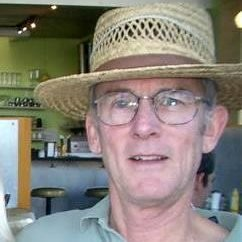
\includegraphics[width=0.25\linewidth]{1516279730868.jpeg}
        \caption{\textbf{Antonin Guttman}}
        \label{fig:enter-label}
  
\end{figure}  

\end{justify}

\end{frame}

\begin{frame}{R-tree}
    \par As árvores R correspondem à estrutura de dados que são utilizadas para indexação de dados multidimensionais, como dados espaciais, por exemplo.

    \begin{figure}[htbp]
    \centering
    \begin{minipage}{0.4\textwidth}
        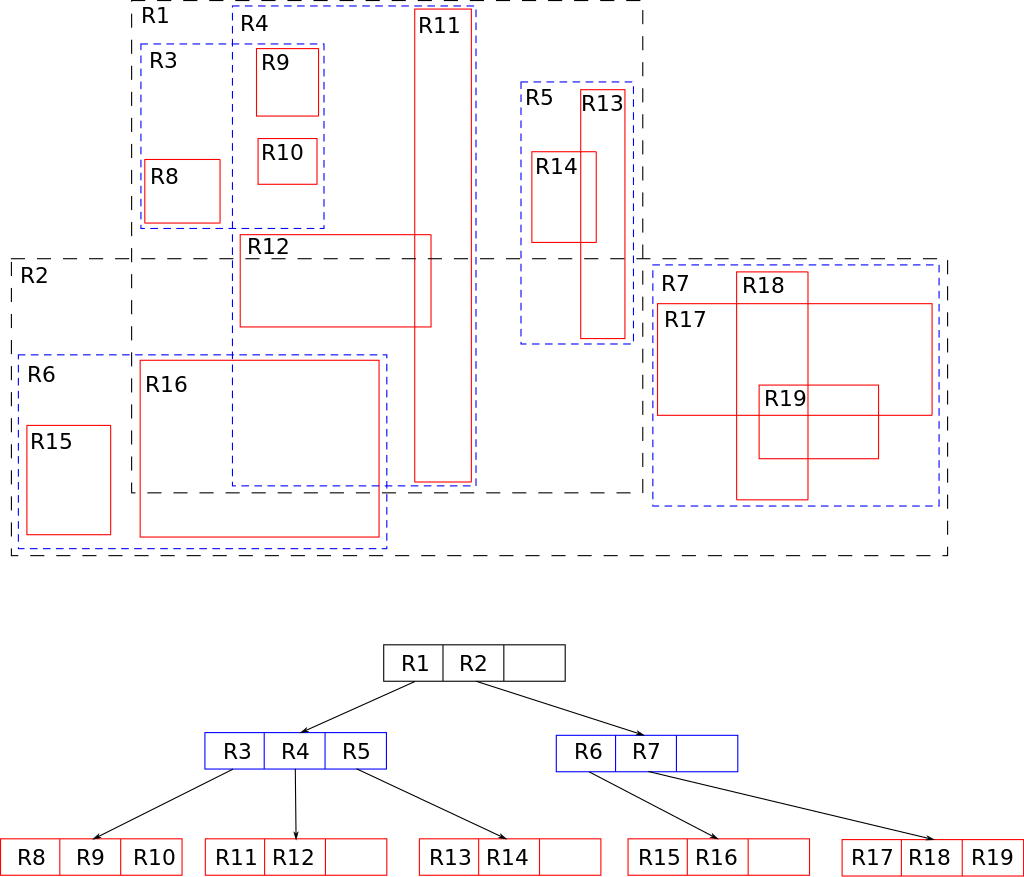
\includegraphics[width=\linewidth]{R-tree.svg.png}
        \caption{\textbf{Árvore R retangular 2D}}
        \label{fig:fig1}
    \end{minipage}\hfill
    \begin{minipage}{0.45\textwidth}
        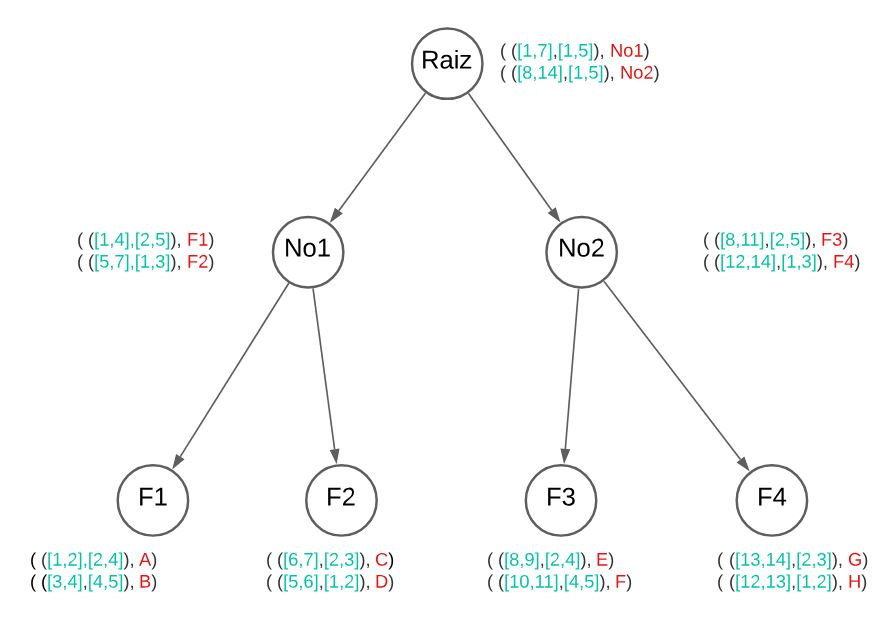
\includegraphics[width=\linewidth]{Rtreeexemplo.JPG}
        \caption{\textbf{Árvore R com intervalos}}
        \label{fig:fig2}
    \end{minipage}
    \end{figure}
\end{frame}

\begin{frame}{O que são Dados multidimensionais?}

    \begin{justify}
    Dados multidimensionais correspondem a um conjunto de informações organizadas em mais de uma variável ou dimensão. Cada dimensão diz respeito a um atributo do dado, podendo, por exemplo, ser algo de natureza escalar, como uma coordenada em um espaço, ou categórica, permitindo uma representação mais complexa da informação.
    \end{justify}
    
    \begin{center}
          \begin{block}{Exemplos de dados multidimensionais (dados espaciais)}
                \begin{itemize}
                        \item \textbf{Ponto}: coordenadas de uma unidade mínima em um espaço.
                        \item \textbf{Linha}: sequência de pontos em uma mesma reta.
                        \item \textbf{Linha poligonal}: sequência de pontos que não se encontram em uma mesma reta.
                        \item \textbf{Poliedro}: sólido composto por faces.
                        \item \textbf{Polígono}: sequência composta por linhas poligonais.
                \end{itemize}
        \end{block}
    \end{center}
\end{frame}


\begin{frame}{Estrutura geral}
    \begin{justify}
        \begin{itemize}
        \item Árvore R de ordem (m, M)
        \item Número máximo de entradas por nó: M
        \item Número mínimo de entradas por nó: m <= |M/2|
        \item Altura máxima da árvore: Hmax = [log\textsubscript{m}N] - 1, onde N é o número de objetos inseridos
     \end{itemize}
    \end{justify}
\end{frame}

\section{Estrutura em C}
\begin{frame}{Representação da estrutura em C}
   \begin{figure}[] 
        \centering
        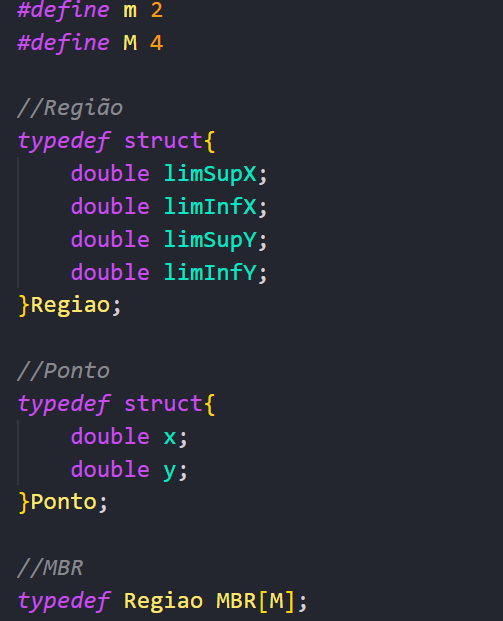
\includegraphics[width=0.33\linewidth]{code1.png}
        \caption{\textbf{Código em C - Parte 1}}
        \label{fig:enter-label}
  
\end{figure}
\end{frame}

\begin{frame}{Representação da estrutura em C}
   \begin{figure}[] 
        \centering
        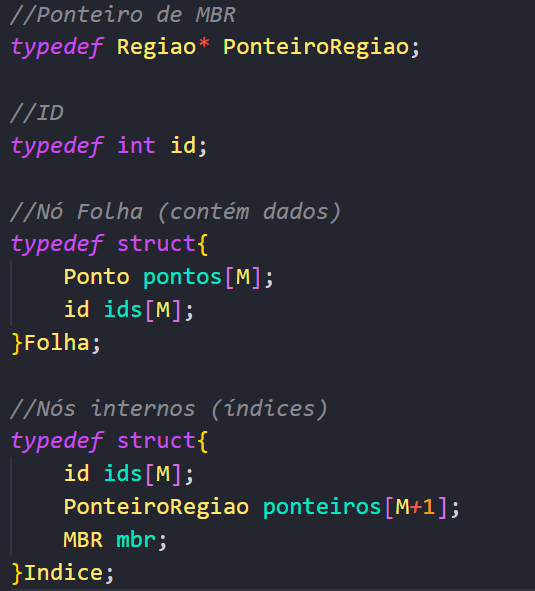
\includegraphics[width=0.33\linewidth]{code2.png}
        \caption{\textbf{Código em C - Parte 2}}
        \label{fig:enter-label}
  
\end{figure}
\end{frame}

\section{Propriedades}
\begin{frame}{MBR (Minimum bounding rectangle)}
    \begin{justify}
        MBR é um protocolo usado pela Árvore R, que visa construir os menores retângulos possíveis em torno dos dados da árvore.

        \begin{minipage}{0.45\linewidth}
            \centering
            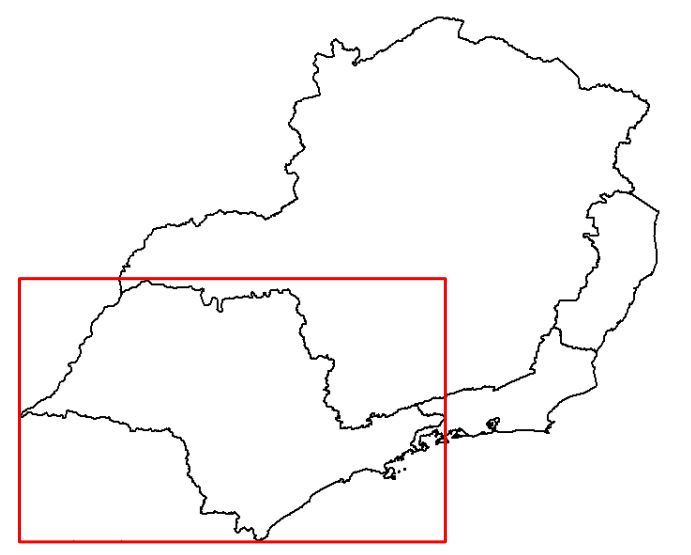
\includegraphics[width=\linewidth]{mbr.JPG}
            
        \end{minipage}
        \hfill
        \begin{minipage}{0.45\linewidth}
            \centering
            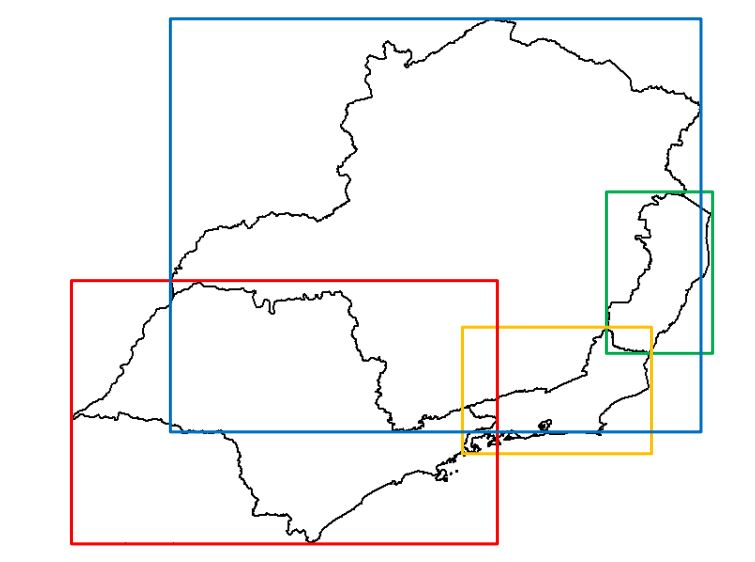
\includegraphics[width=\linewidth]{mbr2.JPG}
            
        \end{minipage}
    \end{justify}
\end{frame}

\begin{frame}{Outros protocolos para representação dos dados multidimensionais}
\begin{figure}[]
        \centering
        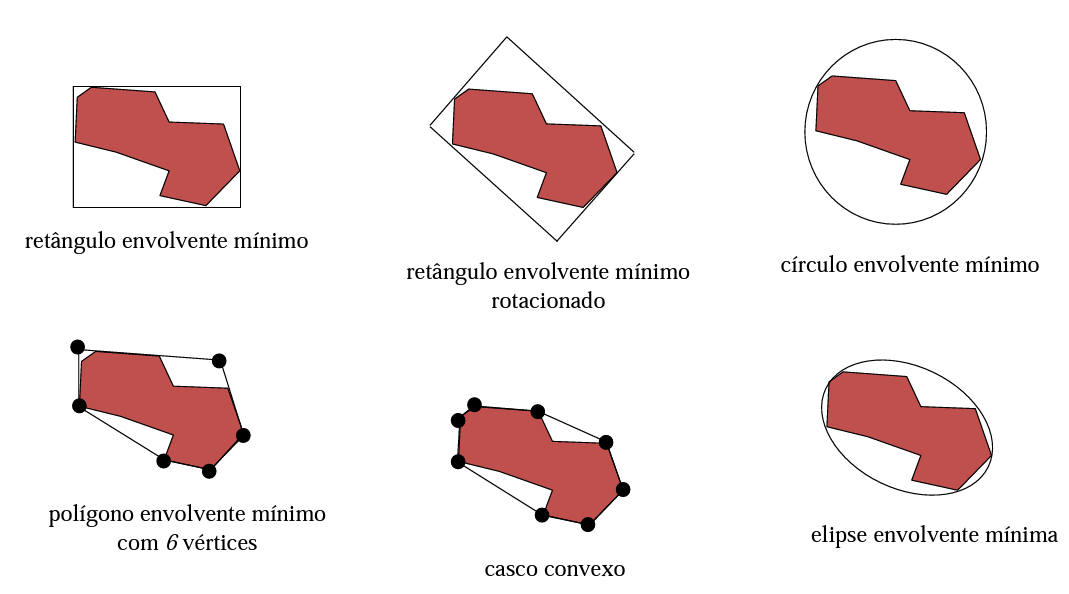
\includegraphics[width=0.75\linewidth]{shapes.png}
        \caption{\textbf{Outras formas conservativas}}
        \label{fig:enter-label}
\end{figure}

\end{frame}
\begin{frame}{Propriedades e características}
    \begin{justify}
     \begin{itemize}
        \item   Possui uma única raiz, nodos internos e nodos folha.
        \item   A raiz aponta para a maior região no domínio espacial.
        \item   Os nodos filhos têm  suas regiões completamente sobrepostas às regiões de seus nodos pais.
        \item   Os nodos folha contêm dados referentes ao MBR para os objetos atuais.
        \item   Todos os nodos folha estão no mesmo nível, semelhante à árvore B.
        \item  O número mínimo de entradas permitindo na raiz é 2, a menos que a raiz seja um nodo folha, nesse caso, ele pode conter uma ou nenhuma entrada, semelhante à árvore B*.
     \end{itemize}
    \end{justify}
\end{frame}

\begin{frame}{Propriedades e características}
    \begin{justify}
     \begin{itemize}
        \item   Construção Bottom-Up: Todos os dados são inseridos nos nodos folha.
        \item   Dinâmica: Permite inserção, remoção e edição dos dados.
        \item   Trabalha com memória secundária: Nodos são páginas de disco com tamanho pré- determinado.
     \end{itemize}
    \end{justify}
\end{frame}


\section{Aplicações}

\begin{frame}{Aplicações da R-tree}
    
    \begin{justify}
        \begin{itemize}
            \item Sistemas de Informações Geográficas (GIS)
            \item Gerenciamento de Dados de Localização
            \item Banco de Dados Espaciais
            \item Detecção de Colisão e Simulações Físicas
            \item Planejamento de Rotas e Otimização Logística
        \end{itemize}
    \end{justify}
\end{frame}

\section{Pesquisa}

\begin{frame}{Pesquisa na R-Tree}
    
    \begin{justify}
        \par Tipos de pesquisas
        \begin{figure}[] 
        \centering
        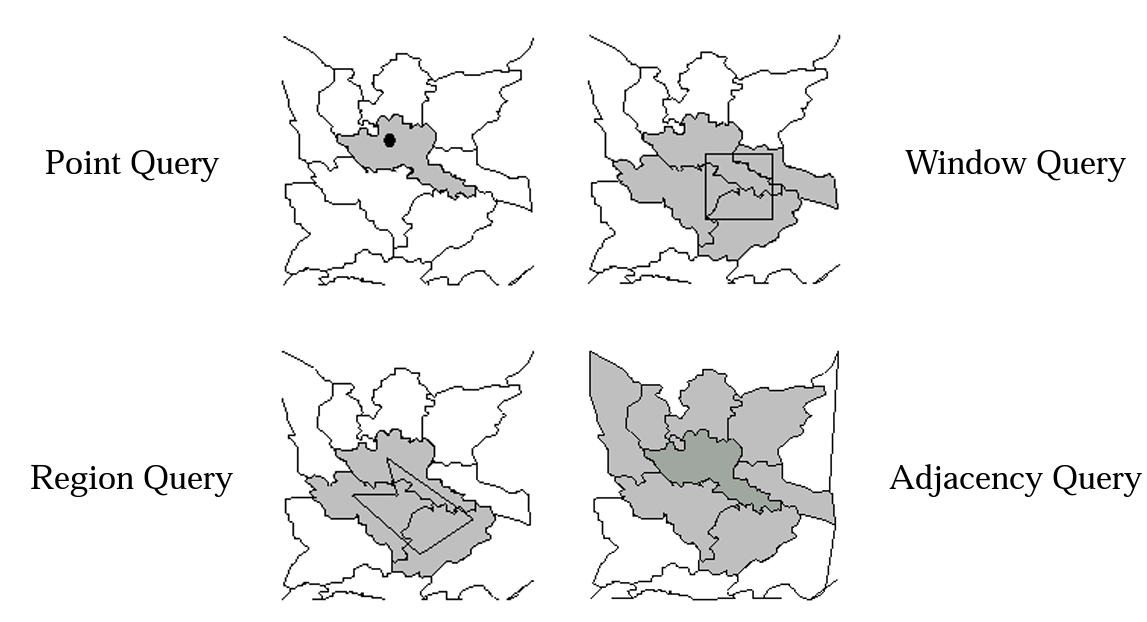
\includegraphics[width=0.71\linewidth]{buscas.png}
        \caption{\textbf{Tipos de pesquisas}}
        \label{fig:enter-label}
  
        \end{figure}
    \end{justify}
\end{frame}

\begin{frame}{Algoritmo de pesquisa}
    \par \textbf{Pesquisando dado específico ou dados em um espaço arbitrário}
    \begin{itemize}
        \item O processo inicia-se verificando se alguma área, presente na raiz, sobrepõe o espaço a ser pesquisado.
        \item Caso haja sobreposição, as áreas presentes nos nodos filhos também são verificadas e, caso haja sobreposição novamente, o processo se dá recursivamente.
        \item O processo recursivo encerra quando chega-se a um nodo folha. A partir daí, verifica-se todas as entradas que interceptam o espaço desejado e as retorna.
    \end{itemize}
    \par \textbf{Complexidade de tempo}
    \begin{itemize}
        \item Caso médio = O(log\textsubscript{m}N)
        \item Pior caso = O(n)
    \end{itemize}
\end{frame}

\begin{frame}{Exemplo 1 de pesquisa}
\begin{figure}[] 
        \centering
        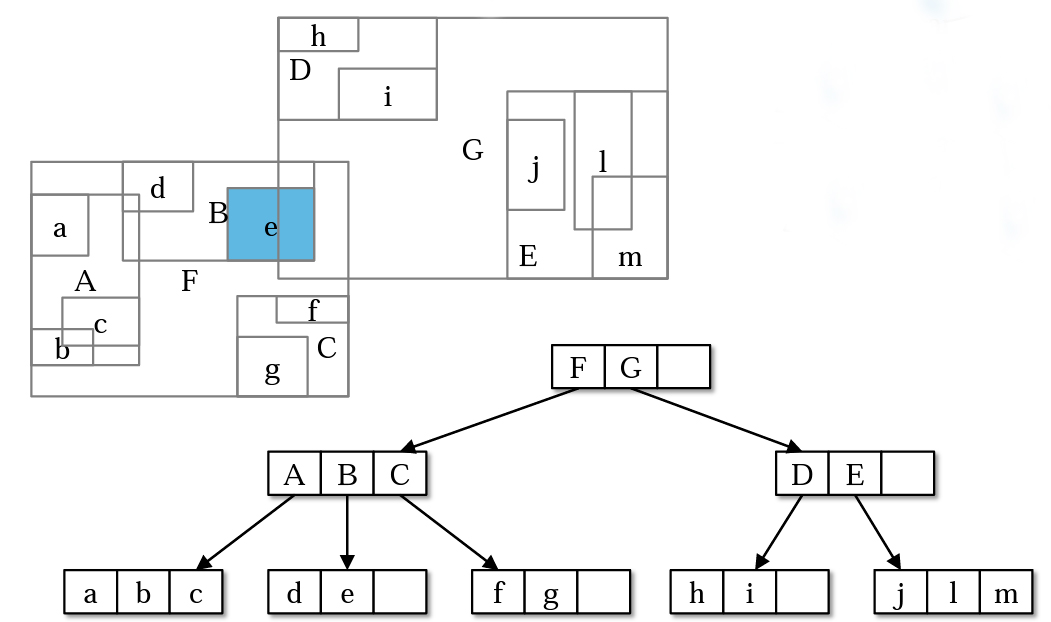
\includegraphics[width=0.73\linewidth]{pesquisa.png}
        \caption{\textbf{Pesquisar o subespaço E dentro da R-tree}}
        \label{fig:enter-label}  
\end{figure}
\end{frame}

\begin{frame}{Exemplo 2 de pesquisa}
\begin{figure}[] 
        \centering
        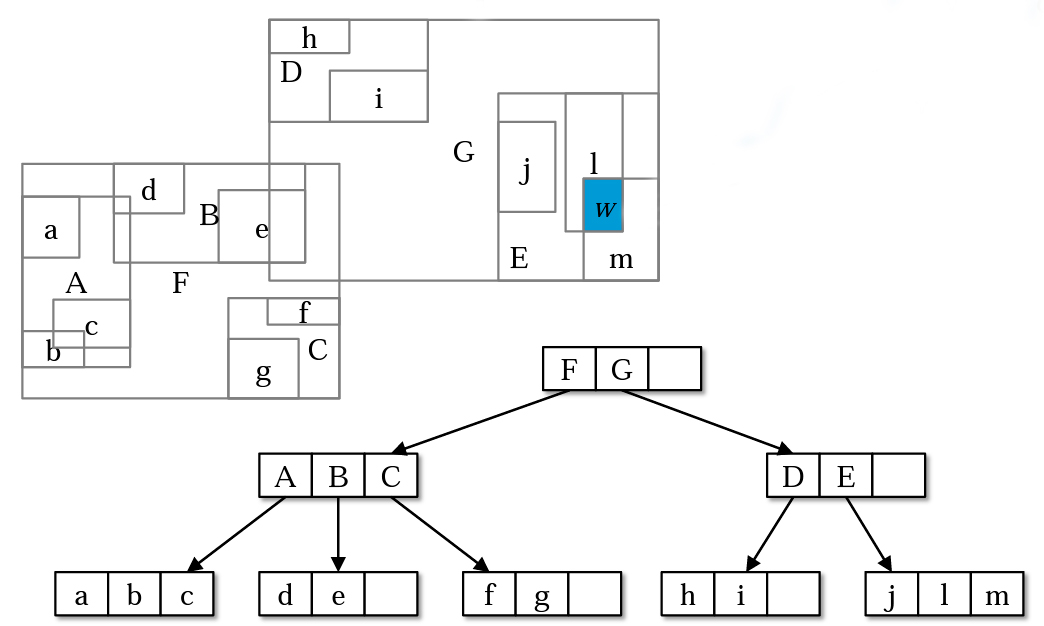
\includegraphics[width=0.73\linewidth]{pesquisa2.png}
        \caption{\textbf{Pesquisar dados dentro de um subespaço w arbitrário}}
        \label{fig:enter-label}  
\end{figure}
\end{frame}

\section{Inserção}

\begin{frame}{Inserção na R-tree}
    
    \begin{justify}
        \begin{itemize}
            \item A árvore é percorrida, desde o nodo raiz até o nodo folha mais apropriado.
            \item Essa escolha é feita a partir do MBR que ocasionará no menor aumento possível da área, que ocorre caso a região do dado esteja fora dos limites de uma área.
            \item Em caso de empates, os métodos de desempate na ordem de prioridade são:
                \begin{itemize}
                    \item Escolher o de menor área
                    \item Escolher aquele com o menor número de entradas
                    \item Escolher arbitrariamente, qualquer um.
                \end{itemize}
            \item Caso o nodo folha contenha espaço suficiente, a nova entrada é inserida no mesmo e o processo de inserção é encerrado.
        \end{itemize}
    
    \end{justify}
\end{frame}

\begin{frame}{Exemplo 1 de inserção parte 1}
\begin{figure}[] 
        \centering
        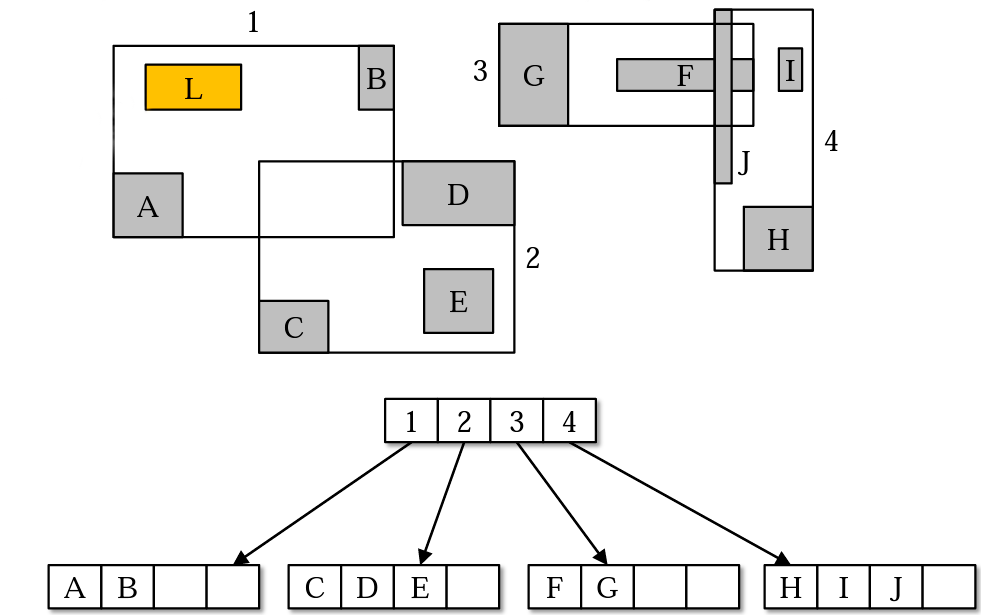
\includegraphics[width=0.65\linewidth]{insercao.png}
        \caption{\textbf{Inserir dado L em uma região já constituída (sem necessidade de criar ou dividir em novos espaços)}}
        \label{fig:enter-label}  
\end{figure}
\end{frame}

\begin{frame}{Exemplo 1 de inserção parte 2}
\begin{figure}[] 
        \centering
        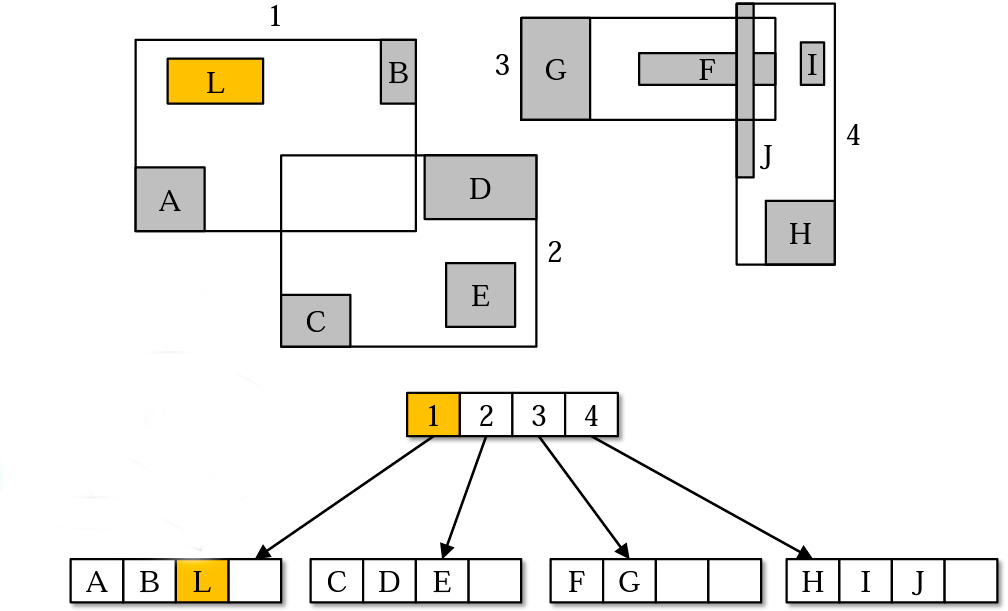
\includegraphics[width=0.65\linewidth]{insercao2.jpg}
        \caption{\textbf{Inserir dado L em uma região já constituída (sem necessidade de criar ou dividir em novos espaços)}}
        \label{fig:enter-label}  
\end{figure}
\end{frame}

\begin{frame}{Exemplo 2 de inserção parte 1}
\begin{figure}[] 
        \centering
        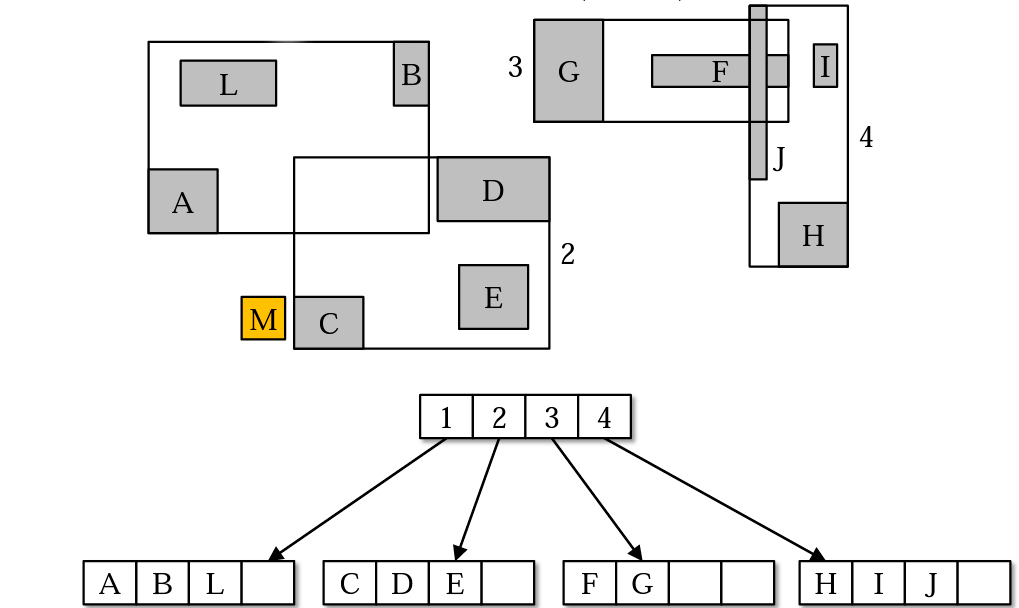
\includegraphics[width=0.65\linewidth]{insercao3.jpg}
        \caption{\textbf{Inserir um dado M em que uma área terá que expandir para agrupá-lo)}}
        \label{fig:enter-label}  
\end{figure}
\end{frame}

\begin{frame}{Exemplo 2 de inserção parte 2}
\begin{figure}[] 
        \centering
        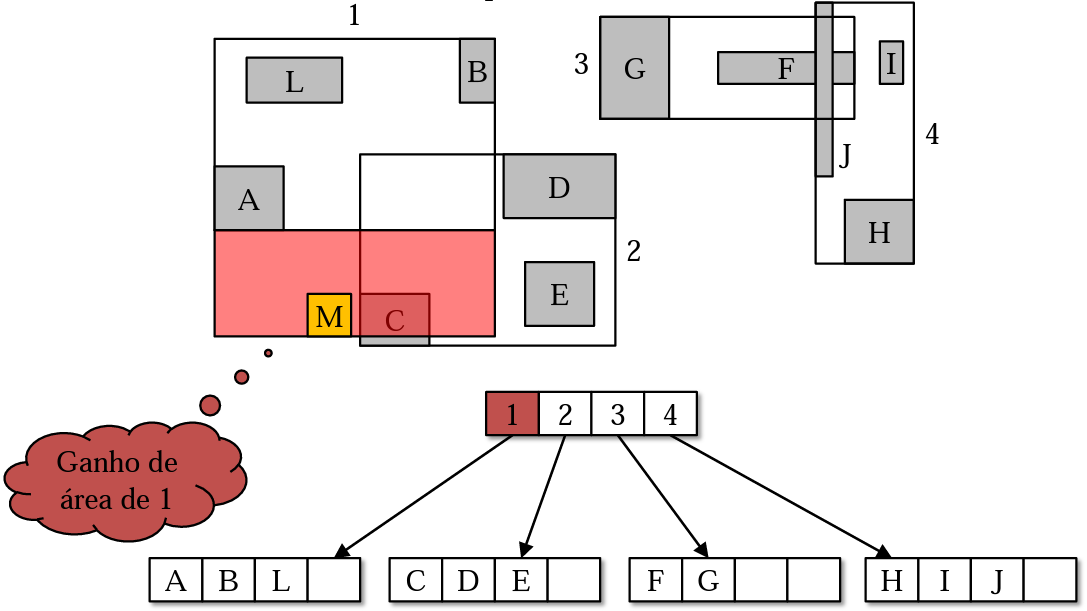
\includegraphics[width=0.65\linewidth]{insercao4.png}
        \caption{\textbf{Inserir um dado M em que uma área terá que expandir para agrupá-lo)}}
        \label{fig:enter-label}  
\end{figure}
\end{frame}

\begin{frame}{Exemplo 2 de inserção parte 3}
\begin{figure}[] 
        \centering
        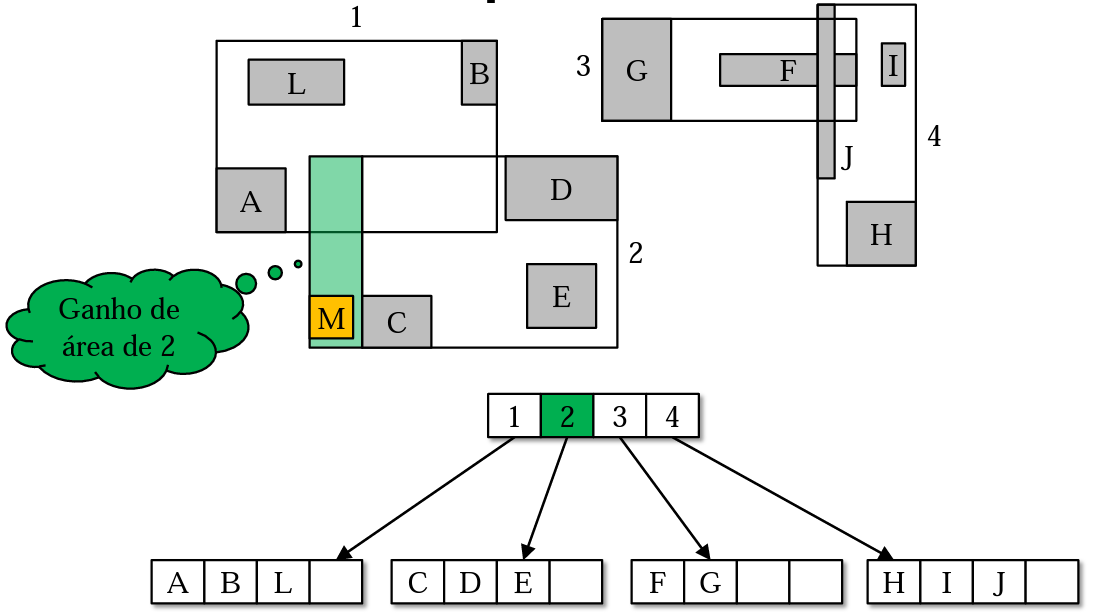
\includegraphics[width=0.65\linewidth]{insercao5.png}
        \caption{\textbf{Inserir um dado M em que uma área terá que expandir para agrupá-lo)}}
        \label{fig:enter-label}  
\end{figure}
\end{frame}

\begin{frame}{Exemplo 2 de inserção parte 4}
\begin{figure}[] 
        \centering
        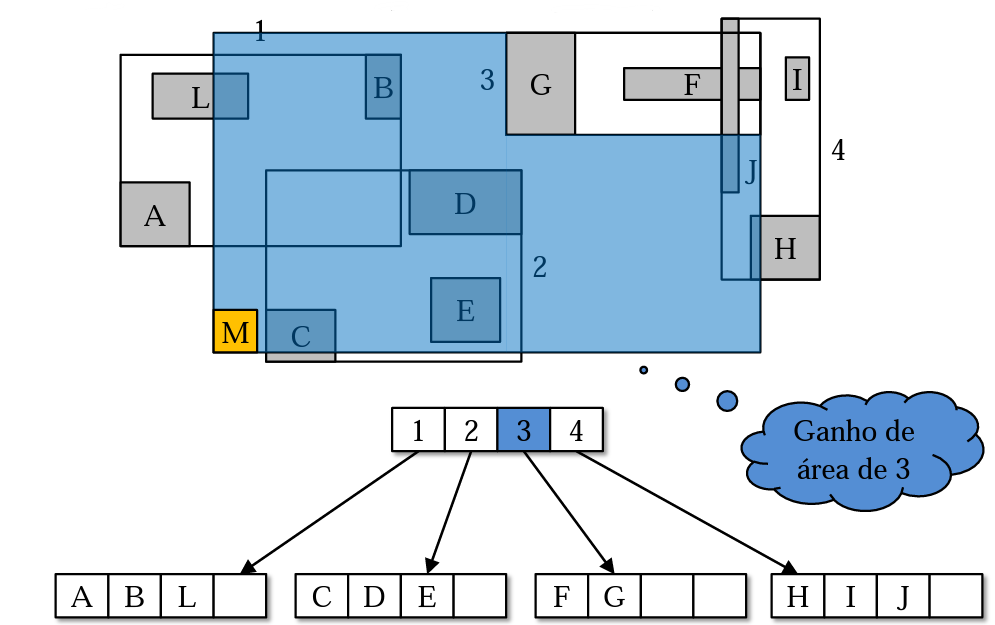
\includegraphics[width=0.65\linewidth]{insercao6.png}
        \caption{\textbf{Inserir um dado M em que uma área terá que expandir para agrupá-lo)}}
        \label{fig:enter-label}  
\end{figure}
\end{frame}

\begin{frame}{Exemplo 2 de inserção parte 5}
\begin{figure}[] 
        \centering
        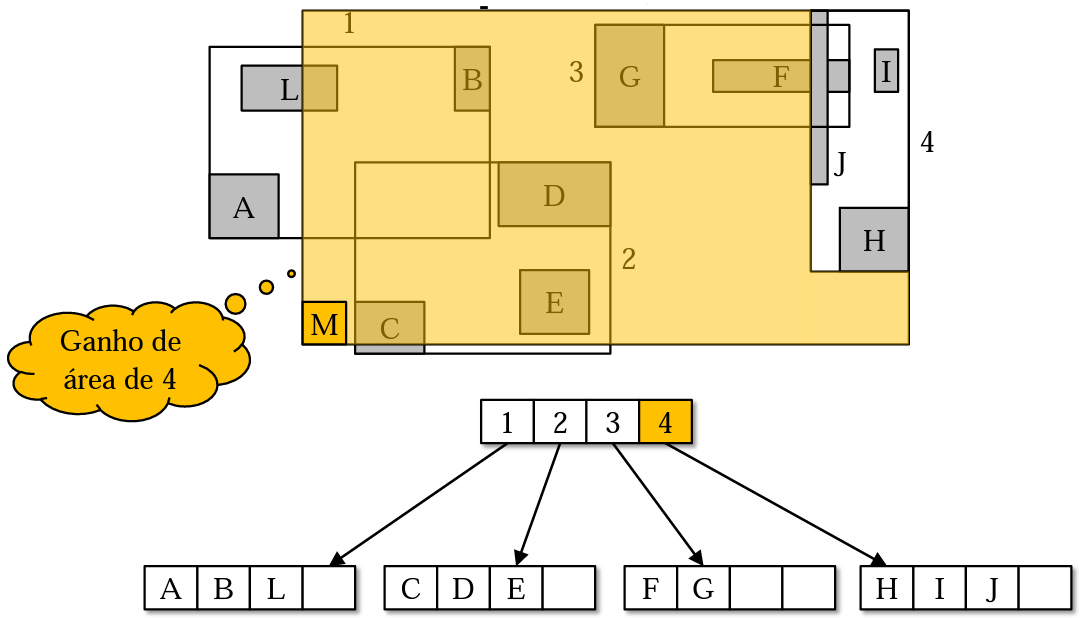
\includegraphics[width=0.65\linewidth]{insercao7.png}
        \caption{\textbf{Inserir um dado M em que uma área terá que expandir para agrupá-lo)}}
        \label{fig:enter-label}  
\end{figure}
\end{frame}

\begin{frame}{Exemplo 2 de inserção parte 6}
\begin{figure}[] 
        \centering
        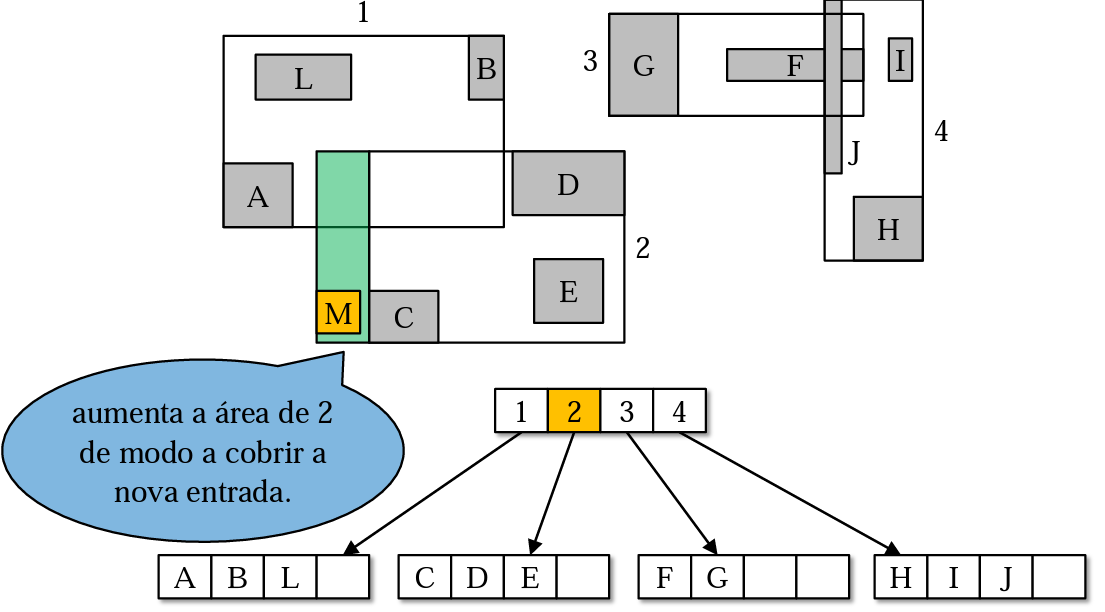
\includegraphics[width=0.65\linewidth]{insercao8.png}
        \caption{\textbf{Inserir um dado M em que uma área terá que expandir para agrupá-lo)}}
        \label{fig:enter-label}  
\end{figure}
\end{frame}

\begin{frame}{Exemplo 2 de inserção parte 7}
\begin{figure}[] 
        \centering
        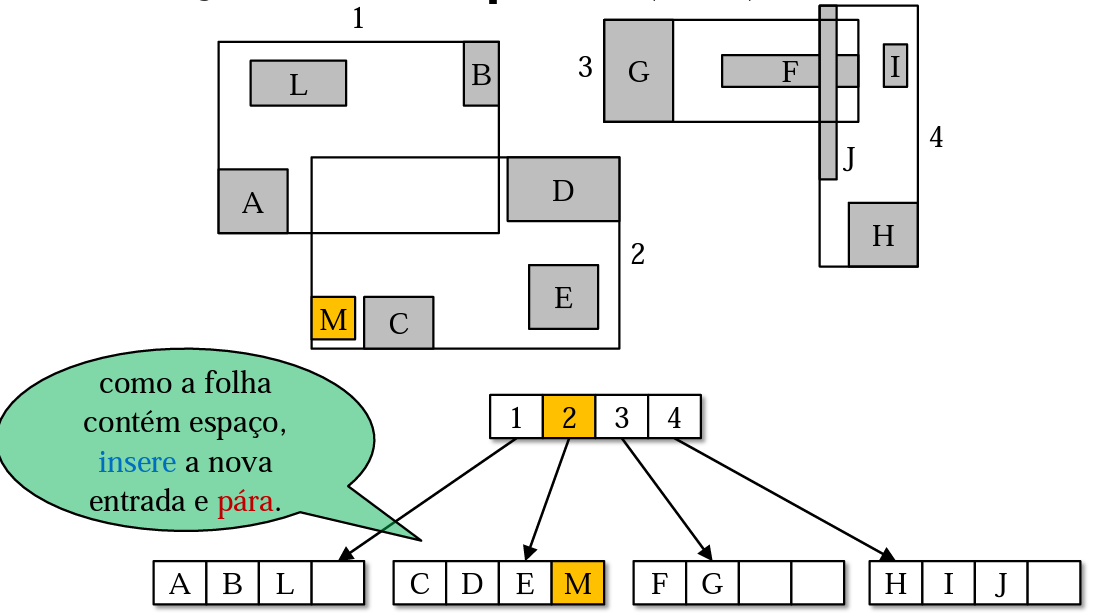
\includegraphics[width=0.65\linewidth]{insercao9.png}
        \caption{\textbf{Inserir um dado M em que uma área terá que expandir para agrupá-lo)}}
        \label{fig:enter-label}  
\end{figure}
\end{frame}



\begin{frame}{Inserção na R-tree}
    \begin{justify}
        \begin{itemize}
            \item Caso o nodo folha F não tenha espaço, ele é \textit{splitado} (dividido) em 2, F1 e F2.
                \begin{itemize}
                    \item A entrada de F no seu nodo pai (P) é ajustada de modo que seu MBR cubra apenas F1.
                    \item É adicionada uma entrada em P para F2. Este passo pode fazer com que o nó P seja \textit{splitado} recursivamente.
                \end{itemize}
            \item As alterações são propagadas para os níveis superiores.
        \end{itemize}
    \end{justify}
\end{frame}

\begin{frame}{Split: Algoritmo Quadrático}
    \par Parte 1: Seleção das seeds
    \begin{itemize}
        \item Seleciona dois objetos como seeds de modo que esses objetos, se colocados juntos, criam o maior dead space possível.
        \begin{itemize}
            \item Dead space: área restante no MBR desconsiderando as seeds.
            \item Dead space (A, B) = Área(MBR(A, B)) - Área (A) - Área (B)
        \end{itemize}
        \item Complexidade: O(M²)
    \end{itemize}

    \par Parte 2: Redistribuição das M-1 entradas
    \begin{itemize}
        \item Até que não reste mais entradas (O(M)), selecionar a entrada cuja diferença de dead space para cada um dos dois nodos N1 e N2 seja máxima (O(M²)).
        \item Inserir a entrada no nodo que requer o menor aumento de seu MBR (O(1)).
    \end{itemize}

    \par Complexidade total de tempo: O(M²).
\end{frame}

\begin{frame}{Split: Algoritmo Exaustivo}
    \begin{justify}
        \item Tal algoritmo de divisão de nós pode-se fazer uma analogia com um algoritmo de força bruta, no qual ele irá testar todos os agrupamentos possíveis para encontrar o menor aumento de MBRs e área de sobreposição.
        \item Possui uma complexidade de tempo de O(2$^{M-1}$)
    \end{justify}
\end{frame}

\begin{frame}{Split: Algoritmo Linear}
    \begin{justify}
        \begin{itemize}
            \item Para cada dimensão, encontra a entrada com o maior tamanho lateral e o menor tamanho vertical, normalizando os valores 
        
            \item Escolhe os dois objetos mais distantes entre si no nodo cheio, ou seja, os com o maior valor normalizado. Esses objetos serão os representantes dos novos nodos após a divisão.

            \item Distribua os objetos restantes entre os dois grupos, atribuindo cada objeto ao grupo com o representante mais próximo.

            \item Crie dois novos nodos e coloque os objetos nos grupos correspondentes nesses nodos.
        \end{itemize}
    \end{justify}
\end{frame}

\begin{frame}{Algoritmo Linear}

        \centering
        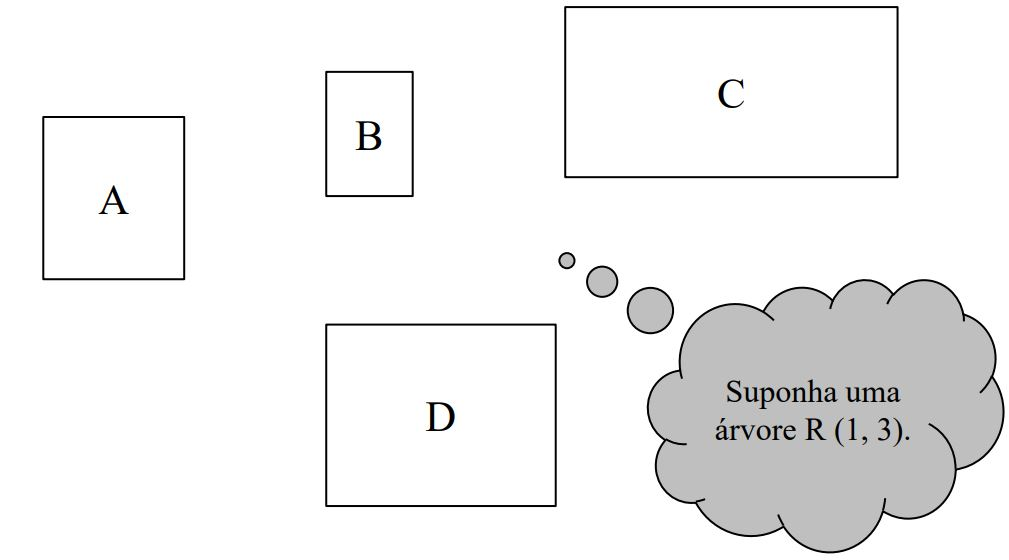
\includegraphics[width=0.75\linewidth]{inser.JPG}
        \label{fig:enter-label}
        
\end{frame}
\begin{frame}{}

        \centering
        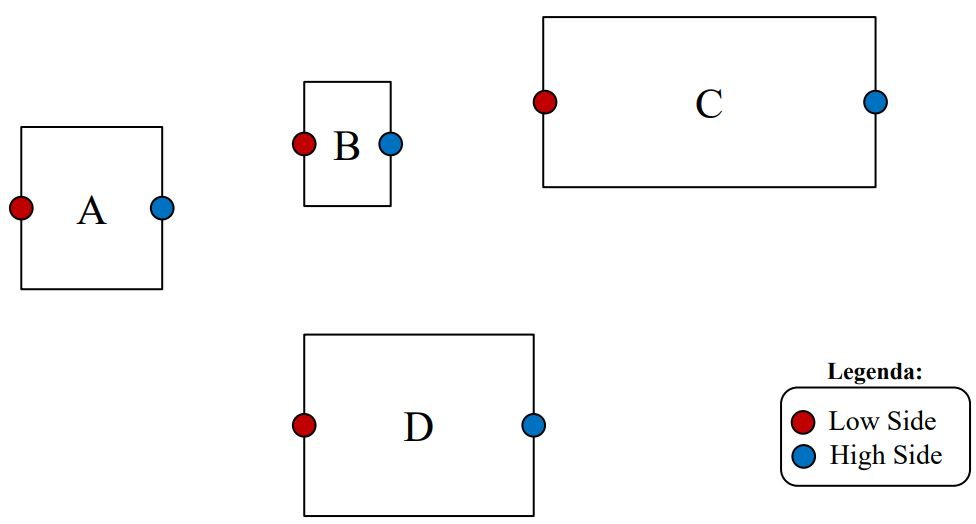
\includegraphics[width=0.75\linewidth]{split1.jpg}
        \label{fig:enter-label}
        
\end{frame}

\begin{frame}{}

        \centering
        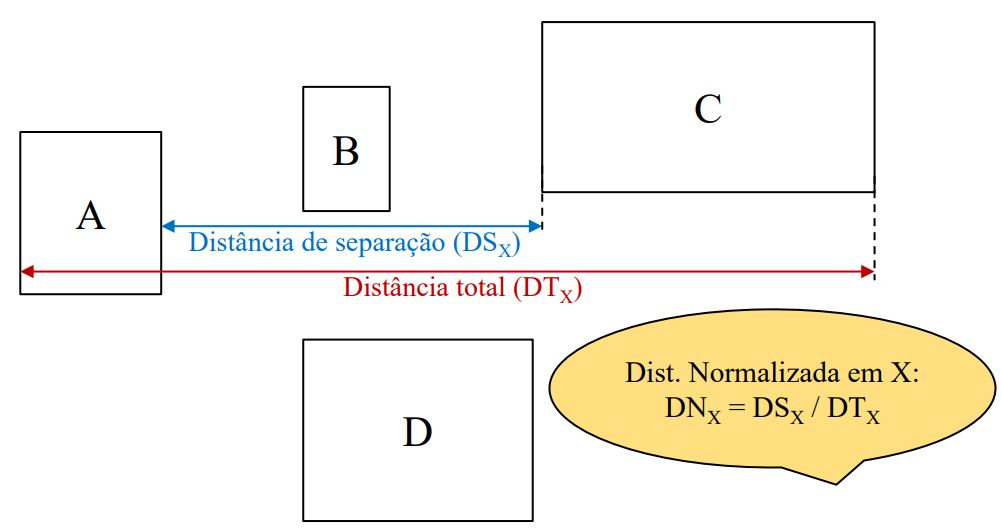
\includegraphics[width=0.75\linewidth]{split3.JPG}
        \label{fig:enter-label}
        
\end{frame}



\begin{frame}{}

        \centering
        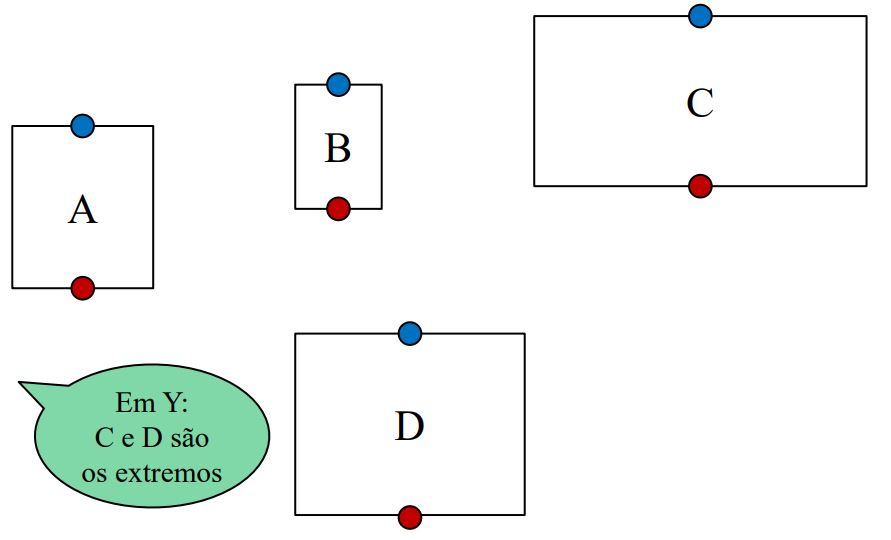
\includegraphics[width=0.75\linewidth]{split4.JPG}
        \label{fig:enter-label}
        
\end{frame}

\begin{frame}{}

        \centering
        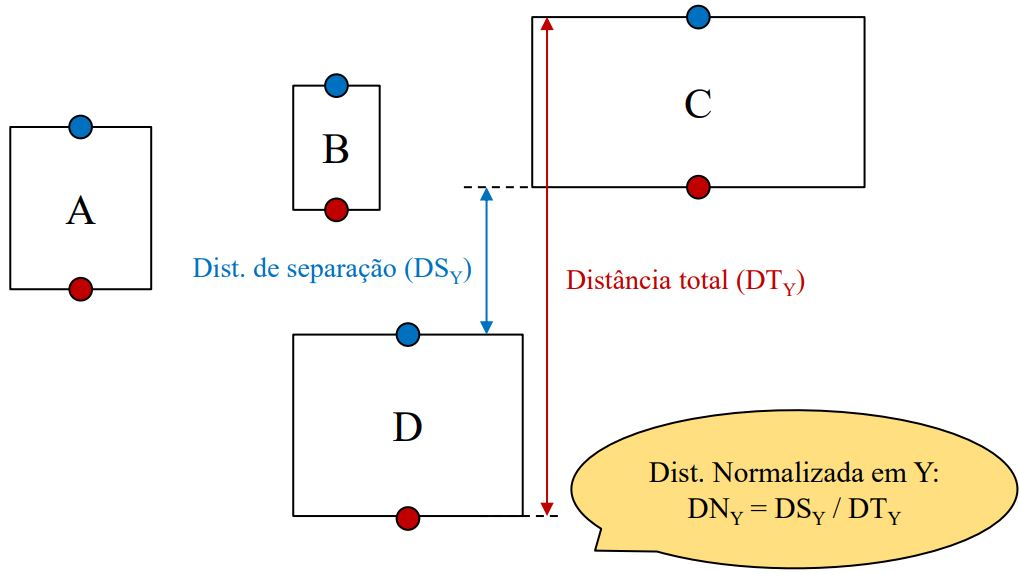
\includegraphics[width=0.75\linewidth]{split5.JPG}
        \label{fig:enter-label}
        
\end{frame}

\begin{frame}{}

        \centering
        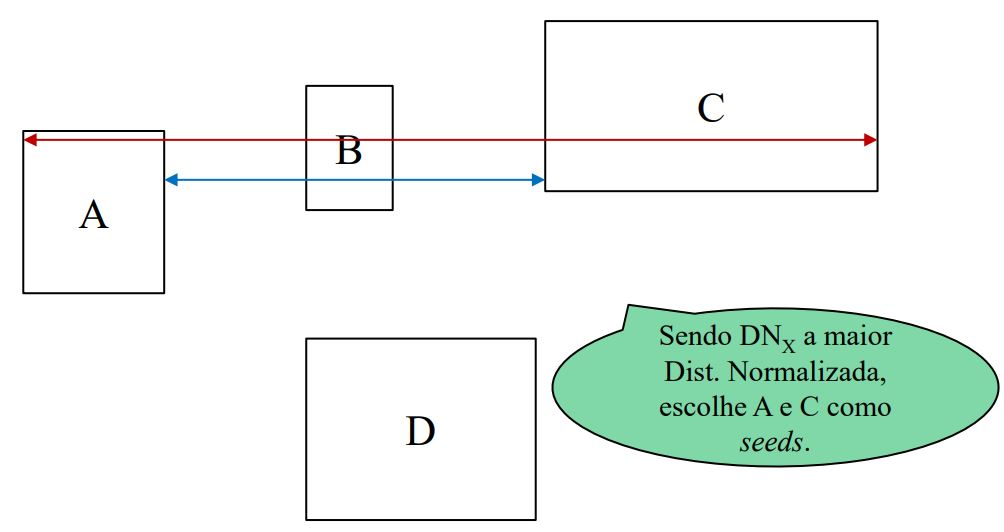
\includegraphics[width=0.75\linewidth]{slit2.JPG}
        \label{fig:enter-label}
        
\end{frame}

\begin{frame}{}

        \centering
        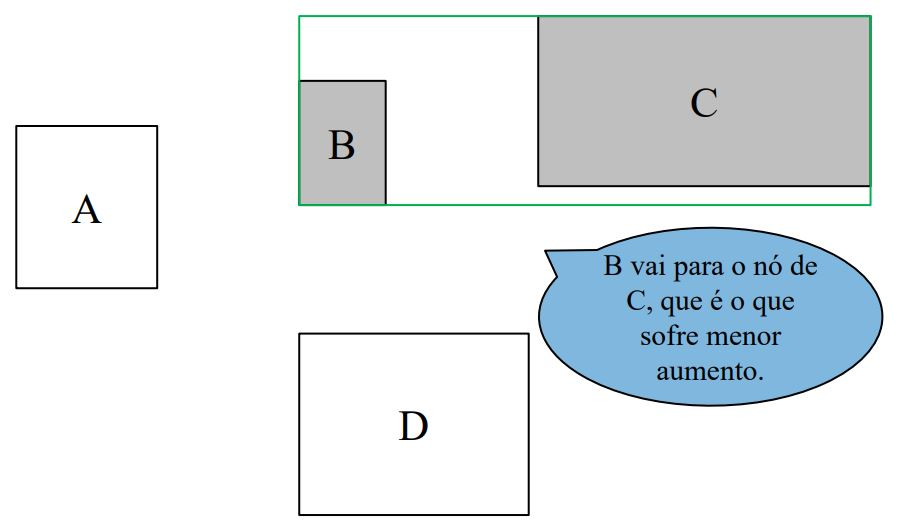
\includegraphics[width=0.75\linewidth]{split6.JPG}
        \label{fig:enter-label}
        
\end{frame}

\begin{frame}{}

        \centering
        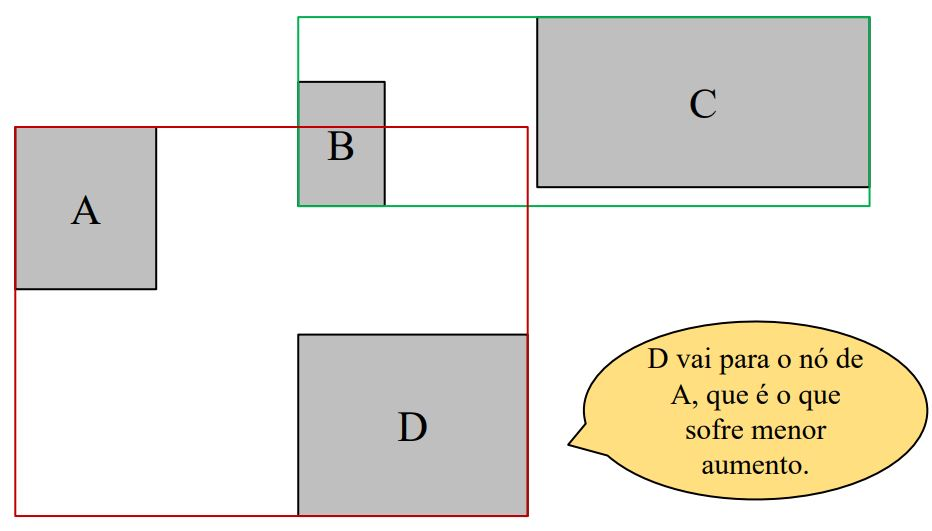
\includegraphics[width=0.75\linewidth]{split7.JPG}
        \label{fig:enter-label}
        
\end{frame}

\begin{frame}{}

        \centering
        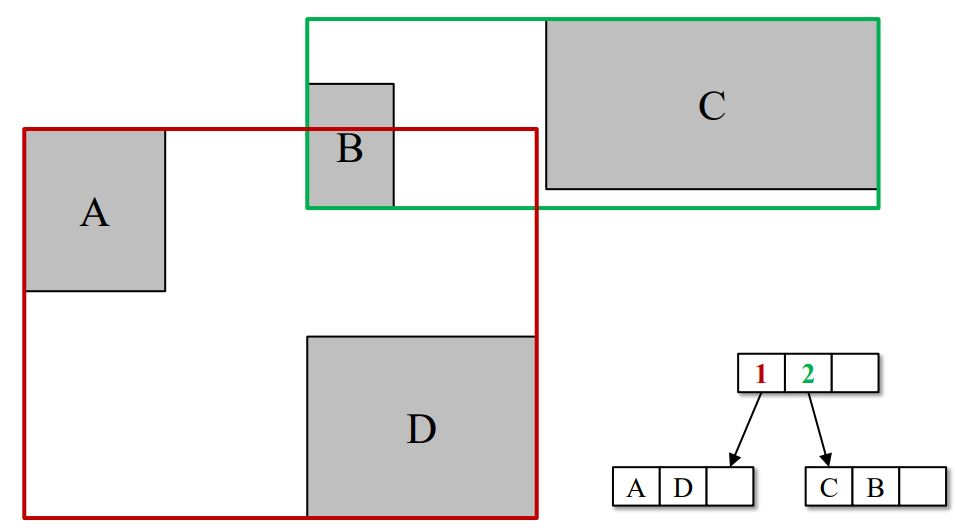
\includegraphics[width=0.75\linewidth]{split8.JPG}
        \label{fig:enter-label}
        
\end{frame}


\section{Variações da R-tree}
\begin{frame}{Variações da Árvore R}
\begin{justify}
    \par Com o tempo, várias variações e aprimoramentos da árvore R foram desenvolvidas para deixar ela top de linha. Dentre elas:
    \begin{itemize}
        \item Árvore R de prioridade
        \item Árvore R*
        \item Árvore R+
        \item Árvore R Hilbert
        \item Árvore X
    \end{itemize}
    \end{justify}

\end{frame}

\section{Desvantagens}
\begin{frame}{Limitações da R-tree}
    
    \begin{justify}
        \begin{itemize}
            \item Quando ocorre a sobreposição de caixas delimitadores, é preciso verificar mais ramificações para encontrar o item desejado e isso aumenta o custa da consulta, levando a um processo mais lento.
            \item A implementação do algoritmo da R-Tree é complexo, já que é necessário usar algumas estratégias para manter o balanceamento da arvore e assim evitar ao máximo a sobreposição.
            \item Há uma dificuldade desta estrutura de dados, em lidar com dados de alta dimensão. Apesar de teoricamente a R-Tree suportar tais dados, isso diminui a performance porque aumenta o numero de dimensões da arvore, aumentando a possibilidade de sobreposição das caixas.
        \end{itemize}
    \end{justify}
\end{frame}

\section{Referências}
\begin{frame}{Referências utilizadas}
    
    \begin{justify}
        \begin{itemize}
           \item MANOLOPOULOS, Y.; NANOPOULOS, A.; PAPADOPOULOS, A. N.; THEODORIDIS, Y. R-Trees: Theory and Applications. Springer, 2006. 
           \item KAO, M.-Y. Encyclopedia of Algorithms. Springer, 2008.
           \item Introduction to R tree. GeeksforGeeks. Disponível em: <https://www.geeksforgeeks.org/introduction-to-r-tree/>. Acesso em: 17 ago. 2023.
           \item WIKIPEDIA CONTRIBUTORS. R-tree. Wikipedia. Disponível em: <https://en.wikipedia.org/wiki/R-tree>. Acesso em: 17 ago. 2023.
        \end{itemize}
    \end{justify}
\end{frame}
\begin{frame}{Referências utilizadas}
    
    \begin{justify}
        \begin{itemize}
           \item Árvore R Luiz Olmes Carvalho SCC 5789 -Base de Dados Profa. Dra. Cristina Dutra de Aguiar Ciferri. [s.l.: s.n., s.d.]. Disponível em: <http://wiki.icmc.usp.br/images/c/cb/SCC578920131-Rtree.pdf>.  Acesso em: 17 ago. 2023.
           \item R-Trees. Cglab.ca. Disponível em: <https://cglab.ca/~cdillaba/comp5409\_project/R\_Trees.html>. Acesso em: 17 ago. 2023.
        \end{itemize}
    \end{justify}
\end{frame}


\end{document}
